\chapter{Paralelné gramatiky}

Skúsme sa trochu zamyslieť nad tým, aký paralelizmus by sme v
gramatikách mohli zaviesť. Jednou z možností by bolo, na rozdiel
od gramatík Chomského hierarchie, kde sa v jednom kroku odvodenia
prepisuje iba jeden neterminál, prepísať naraz všetky neterminály
vo vetnej forme. Inou by mohlo byť prepisovanie rovnakých
neterminálov na jeden krok a ako uvidíme, existuje množstvo
ďalších modifikácií

\section{Lindenmayerove systémy ($L$-systémy)}

\begin{motiv}
%%% {{{
    Pôvodná motivácia, ktorá dala vzniknúť teoretickému modelu, o
    ktorom si teraz niečo bližšie povieme, nebola ani zďaleka taká
    blízka teórii jazykov, ako by si niekto mohol chybne myslieť. Pán
    Lindenmeyer, podľa ktorého je tento model pomenovaný, skúmal
    správanie sa istého druhu fylamentóznych organizmov, ktoré
    vyzerali asi takto: tvorila ich reťaz buniek, pričom každá bunka
    (okrem krajných, ktoré majú po jednom) mala práve dvoch susedov,
    ktorí ju mohli, resp. nemuseli v jej správaní ovplyvňovať. Celý
    mechanizmus fungoval akoby v taktoch tak, že sa niekedy pár buniek
    rozhodlo, že sa rozmnoží (presnejšie, že sa každá z nich
    rozmnoží), niekedy zasa niektoré bunky odumreli, a teda z reťazca
    akoby zmizli a inokedy sa s nimi nič nedialo
%%% }}}    
\end{motiv}

\subsection{$OL$-systémy}

\begin{definicia}[$OL$-systém]
%%% {{{
    Lindenmayerovým $OL$-systémom nazveme
    trojicu $G=(V,P,w)$, kde $V$ je abeceda symbolov,
    $P\subseteq V\times V^{*}$ je množina prepisovacích
    pravidiel takých, že $proj_{1}(P)=V$ 
    (teda musí existovať pravidlo pre každý symbol abecedy $L$-systému)
    a $w\in V^{+}$ nazývame axiom, alebo
    počiatočné slovo.\footnote{Je dobré si hneď na začiatku uvedomiť
        rozdiel medzi $L$-systémami a gramatikami, s ktorými sme sa
        stretli v Chomského hierarchii. Počiatočné slovo
        $L$-systému nemusí tvoriť iba jeden symbol, ba dokonca tu
        nerozlišujeme medzi terminálmi a neterminálmi}
%%% }}}        
\end{definicia}

\begin{definicia}[Krok odvodenia]
%%% {{{
    Krok odvodenia v $OL$-systéme je relácia $\odvodenie$ na $V^{*}$ definovaná
    nasledovne: $u\odvodenie v$ práve vtedy, ak $u=a_{1} \dots a_{n}$,
    $\forall i: a_{i} \in V$, $v=b_{1} \dots b_{n}$, 
    $\forall i: b_{i} \in V^{*}$ a 
    $\forall i: a_{i} \pravidlo b_{i} \in P$. 
    Inak povedané, naraz prepíšeme všetky písmená, každé nejakým
    pravidlom.
%%% }}}
\end{definicia}

\begin{definicia}[Jazyk generovaný $OL$-systémom]
%%% {{{
    Jazyk generovaný $OL$-systémom $G$ je 
    $L(G)=\{u\in V^{*} \mm w \odvodeniena{*} u\}$.\footnote{teda prakticky
        každá vetná forma, ktorú z
        počiatočného slova dostaneme (vrátane jeho samého), patrí do
        jazyka $L(G)$, ak $G$ je $L$-systém
        }
%%% }}}        
\end{definicia}

\begin{definicia}[$DOL$-systém]
%%% {{{
    Deterministický $OL$-systém je taký $OL$-systém,
    kde $\forall a\in V$ existuje práve jedno pravidlo
    $a \pravidlo u\in P, u\in V^*$.
%%% }}}    
\end{definicia}

\begin{definicia}[$POL$-systém]
%%% {{{
    Propagating/pokračujúci $OL$-systém je taký $OL$-systém, ktorý
    je bez-$\eps$.\fixme{Znamena to, ze nema epilon alebo ze
        nema epsilonove pravidla}
%%% }}}        
\end{definicia}

\begin{priklad}
%%% {{{ priklad a^{2^n}
    Uvažujme systém $G_1=(\{ a \},\{ a \pravidlo a^2\}, a)$.
    Potom $L(G_1)=\{ a^{2^n} \mm n \ge 0\}$.
    Ukážka odvodzovania slova v tomto OL systéme je na obrázku 
    \ref{img:ol_priklad_1}.
    Ako vidieť, $OL$-systém $G_1$ nám úplne jednoducho 
    (použitím jediného pravidla) umožňuje
    generovať jazyk, na ktorý by nám v Chomského hierarchii
    nestačili ani bezkontextové prostriedky.
    Sila $OL$-systémov spočíva v paralelnom prepisovaní,
    kedy v jednom kroku odvodenia
    musíme použiť prepisovacie pravidlá na všetky symboly.
    Skúsme ale do $G_1$ pridať jedno pravidlo:\\
    $G_{1}'=(\{ a \},\{ a\pravidlo a,
    a \pravidlo a^2 \}, a)$ potom $L_{G_1'}=a^{+}$ a veľká sila je razom
    preč. Je tomu tak preto, lebo pridaním pravidla $a\pravidlo a$ sme
    umožnili akoby rozsynchronizovať odvodenie, a teda symboly sa
    teraz neprepisujú naraz, ale každý v inom čase.

    \begin{figure}[htp]
        \centering
        \includegraphics{img/1paralelne_gramatiky/ol_priklady.1.mps}
        \caption{Príklad generovanie jazyka $a^{2^n}$}
        \label{img:ol_priklad_1}
    \end{figure}
%%% }}}    
\end{priklad}


\begin{priklad}
%%% {{{ fibonacciho postupnost
    Uvažujme systém $G_{2}=(\{a,b\},\{ a \pravidlo b, b \pravidlo ab \},a)$.
    Jazyk $L(G_{2})$ budú
    tvoriť slová, ktorých dĺžky sú členy Fibonacciho postupnosti, ako
    možno vidieť na obrázku \ref{img:ol_priklad_2}. Máme teda
    opäť jeden dosť zložitý, zrejme nie bezkontextový jazyk,
    ktorý dokážeme $OL$-systémom pomerne jednoducho generovať.
    \begin{figure}[htp]
        \centering
        \includegraphics{img/1paralelne_gramatiky/ol_priklady.2.mps}
        \caption{Generovanie Fibonnaciho postupnosťi}
        \label{img:ol_priklad_2}
    \end{figure}
%%% }}}    
\end{priklad}


\begin{priklad}
%%% {{{ stvorce
    Zoberme $G_3=(\{a,b,c\},\{a \pravidlo abcc,b \pravidlo bcc,
        c \pravidlo c\},a)$. Dĺžky
    slov jazyka $L(G_3)$ tvoria postupnosť štvorcov (druhých mocnín)
    prirodzených čísel (obr. \ref{img:ol_priklad_3}).

    \begin{figure}[htp]
        \centering
        \includegraphics{img/1paralelne_gramatiky/ol_priklady.3.mps}
        \caption{Generovanie štvorcov}
        \label{img:ol_priklad_3}
    \end{figure}
%%% }}}
\end{priklad}


\begin{definicia}[$\mathcal{AFL}$]
%%% {{{
    Abstract Family of Languages je každá trieda
    jazykov obsahujúca nejaký neprázdny jazyk, ktorá je uzavretá na
    zjednotenie $\union$, zreťazenie $\cdot$, kladnú iteráciu $^+$,
    nevymazávajúci homomorfizmus $h_{\eps}$,
    inverzný homomorfizmus $h^{-1}$ a prienik s regulárnym jazykom
    $\intersect\mathcal{R}$.
%%% }}}    
\end{definicia}

\begin{veta}
    $\Lang_{OL}$ je anti-$\mathcal{AFL}$ (t.j. nie je uzavretá
    na žiadnu $\mathcal{AFL}$ operáciu)
\end{veta}

\begin{dokaz}
    Pre každú $\mathcal{AFL}$ operáciu ukážeme, že trieda
    $\Lang_{OL}$ na ňu nie je uzavretá

    \begin{itemize}
    \item[$\union:$] Nech $L_1 = \{ a \}, L_2=\{ a^2 \}$.
        Platí $L_1,L_2 \in \Lang_{OL}$ a sporom
        predpokladajme, že $L=L_1 \union L_2 = \{ a, a^2 \}\in \Lang_{OL}$.
        Potom existuje nejaký $OL$-systém $G$, ktorý jazyk $L$
        generuje. Ten ale musí mať nejaký axiom, môžu nastať dve možnosti:
        %%% {{{
        \begin{enumerate}
        \item axiom je $a$ - potom ale v $G$ existuje pravidlo 
            $a\pravidlo a^2$,
            lebo keby neexistovalo, tak by sme slovo $a^2$ nikdy
            nevyrobili, resp. by sme vyrobili iné slová, ktoré do $L$
            nepatria. Keďže máme toto pravidlo, tak môžeme vyrobiť aj slová,
            ktoré do $L$ nepatria (napr. $a^4$), čo je spor s tým, že
            $G$ generuje $L$.

        \item axiom je $a^{2}$ - potom ak z neho chceme vyrobiť $a$, tak
            musíme v $G$ mať pravidlo $a\pravidlo\eps$,
            ale aj $a\pravidlo a$, lebo
            keby sme ho nemali, tak vďaka paralelnému prepisovaniu symbolov by
            sme dostali $\eps \in L$. My ale vieme, že
            $\eps\not\in L$. No a ak tu už máme tieto dve pravidlá, tak
            $\eps$ chtiac-nechtiac niekedy vyrobíme, čo je opäť v spore
            s tým, že $\eps\not\in L$
        \end{enumerate}

        Teda dostávame $L\not\in\mathcal{L}_{OL}$.\footnote{Dostávame sa
        teda k možno trošku prekvapujúcemu výsledku. Ukazuje sa, že i keď
        $L$-systémy v predchádzajúcom texte zvládli taký krkolomný jazyk
        ako bol $L(G_{1})$, neporadia si s evidentne regulárnym jazykom
        obsahujúcim iba dve slová}
        %%% }}}

    \item[$\cdot:$] Zvolíme $L_1=\{a\}\in \Lang_{OL},
        L_2=\{\eps,a\}\in\Lang_{OL}$ ale $L_1 \cdot
        L_2=\{a,a^2\}\not\in \Lang_{OL}$ ako sme v
        predchádzajúcej časti ukázali.

    \item[$ ^+:$] Definujme 
        $L=\{aa\} \union \{ b^{2^n} \mm n \ge 2 \}
            \in\Lang_{OL}$. Dôkaz urobíme sporom -- nech $G$ je
        $OL$-systém pre $L^{+}$:

        \begin{enumerate}
        \item uvedomme si, že axiomom $G$ môže byť jedine $aa$, ak by tomu
            tak nebolo, axiomom by muselo byť $b^{i}$ pre nejaké $i\geq4$.
            To by sme ale nutne museli mať pravidlo $b\pravidlo a$ alebo 
            $b\pravidlo a^2$, lenže potom by sme vyrobili aj slovo tvaru 
            $b^i a^j$ kde  $i,j\neq0$ a  také slovo do jazyka $L^{+}$
            nepatrí.
        \item $\eps \not \in L^{+} \then G$ je $POL$-systém

        \item $a^4 \in L^{+} \then a\pravidlo a^2\in P$ (nesmú tu byť
            pravidlá tvaru $a\pravidlo a,a\pravidlo a^3$,
            pretože by sme mohli vyrobiť
            aj slovo $ab^{i}\not\in L^{+}$)

        \item $a^2 \odvodeniena{*} b^4 \then a\pravidlo b^{i}\in P$ 
            pre $1\le i\le 3$. Ak teraz použijeme 
            $a\pravidlo a^2$ a $a\pravidlo b^{i}$ dostaneme 
            $a^2 \odvodenie a^2 b^i \not\in L^{+}$
        \end{enumerate}

    \item[$h_{\eps}:$] Uvažujme jazyk
        $L=\{\eps,a,a^2\}\in \Lang_{OL}$ a definujme
        homomorfizmus $h$ nasledovne: $h(a)=a^2$, potom
        $h(L)=\{\eps,a^2,a^4\} \not \in \Lang_{OL}$, čo sa
        dokáže rozbitím na prípady podobne ako pre $\union$

    \item[$h^{-1}:$] Uvažujme jazyk $L=\{a\}\in \Lang_{OL}$ a
        homomorfizmus $h$ daný predpisom $h(a)=a^2$. Potom
        $h^{-1}(L)=\emptyset \not\in \Lang_{OL}$

    \item[$\intersect\mathcal{R} :$] Uvažujme jazyk
        $L_1=\{\eps,a,a^2\} \in \Lang_{OL}$ a regulárny
        jazyk $L_2=\{a^3\}^{*}$.
        Dostávame rovnosť $L_1 \intersect
        L_2 =\{\eps\}\not\in \Lang_{OL}$.\footnote{
            $\{\eps\}\not\in\mathcal{L}_{OL}$, pretože každý
            $OL$-systém, ktorý by tento jazyk generoval, by musel mať ako
            axiom $\eps$, čo je z definície axiomu nemožné}
    \end{itemize}
\end{dokaz}

\begin{dosledok}
    $\mathcal{L}_{OL}$ nie je uzavretá na substitúciu ani na
    zobrazenie $a$-prekladačom a nie je uzavretá ani na $\intersect$ a
    $^{C}$ (komplement)
\end{dosledok}

\begin{dokaz}
    Čo sa týka uzavretosti tejto triedy na zobrazenie $a$-prekladačom,
    princíp dôkazu je podobný ako pri predchádzajúcich uzáverových
    vlastnostiach. Keďže $\mathcal{L}_{OL}$ nie je uzavretá na
    $\intersect\mathcal{R}$, tak nemôže byť uzavretá ani na $\intersect$
    všeobecne. Uzavretosť na $^{C}$ nechávame na čitateľa
\end{dokaz}

\begin{veta}
    $\mathcal{L}_{OL}$ je uzavretá na zrkadlový obraz
\end{veta}

\begin{dokaz}
    Idea je rovnaká ako pre bezkontextové gramatiky. Je daný jazyk
    $L$. Nech $G=(V,P,w)$ je $OL$-systém taký, že $L(G)=L$. Zostrojíme
    $OL$-systém $G'=(V',P',w')$ tak, že $V=V'$, ak $a\ra b_{1}\dots
    b_{n}\in P$, potom $a\ra b_{n}\dots b_{1}\in P^{'}$ a ak
    $w=w_{1}\dots w_{m},\forall i\med w_i\in V$, tak $w'=w_{m}\dots
    w_{1}$. Je zrejmé, že $L(G')=L^{R}$
\end{dokaz}

\begin{veta}
    Nech $L\in\mathcal{L}_{OL}$ je jazyk $L\subseteq a^{*}$, potom
    $L^{*}\in\mathcal{L}_{OL}$
\end{veta}

\begin{dokaz}
    Nech $L=L(G)$ kde $G=(\{a\},P,a^{m}),m\geq1$

    \begin{enumerate}
    \item $L$ je konečný:
        \begin{enumerate}
        \item $L=\{a\}$ alebo $L=\{\eps,a\}\rightsquigarrow
            L^{*}=a^{*}\in\mathcal{L}_{OL}$
        \item nech $L=\{w_{1},\dots,w_{n}\}$, kde
            $w_{1}\neq\eps,w_{1}\neq a$ (jazyk musí obsahovať slovo
            dlhšie ako $|a|$), potom $L^{*}=L(G')$, kde $G'=(\{a\},\{a\ra
            w_{1},\dots,a\ra w_{n},a\ra\eps\},w_{1})$
        \end{enumerate}

    \item $L$ je nekonečný: $\forall i\med 1\leq i\leq m$ nech
        $v_{i}$ je najkratšie slovo v $L$ také, že $|v_{i}|\cong i\med
        mod\med m$ ak existuje, inak ho nedefinujeme. Nech $G'$ je
        $OL$-systém tvaru $G'=(\{a\},P',a^{m})$, kde
        $P'=\{a\ra\eps\}\union\{a\ra u\mm
        a^{m}\underset{G}\Rightarrow u$ alebo $\exists i\med
        v_{i}\underset{G}\Rightarrow u\}$. Tvrdíme, že $L(G')=L^{*}$

        \begin{description}
        \item{$\subseteq$:} Každé $u$ v pravých stranách $P'$ patrí do
        $L$ a teda všetky slová generované $OL$-systémom $G'$ patria do
        $L^{*}$, pretože začíname z $a^{m}\in L$, v ďalšom kroku prepíšeme
        každý symbol buď na $\eps$ (a teda sa ho zbavíme), alebo ho
        prepíšeme na slovo $\in L$, vetná forma má teda v každom kroku
        tvar $w=w_{1}\dots w_{n},\med\forall i\med i=1\dots n\med w_{i}\in
        L\rightsquigarrow w\in L^{*}$
        \item{$\supseteq$:} Opäť budeme kvôli lepšej zrozumiteľnosti
        rozlišovať dva prípady:
        \begin{description}
        \item{A)} $L\subseteq L(G')$ ukážeme MI vzhľadom na počet krokov
        odvodenia nasledovne:
        \begin{description}
        \item{$1^{\circ}$} $a^{m}\in L$, súčasne $a^{m}\in L(G')$
        \item{$2^{\circ}$} ak $x\in L$ a $x\underset{G}\Rightarrow y$, potom
        $x\underset{G'}\Rightarrow y$, lebo $x=(a^{m})^{j}v_{i}$ pre
        nejaké $i,j$
        \[
        \overbrace{\underbrace{aa\dots a}_{m}\underbrace{aa\dots
        a}_{m}\dots\underbrace{aa\dots a}_{m}
        \underbrace{\underbrace{aa\dots a}_{m}\dots\underbrace{aa\dots
        a}_{m}\underbrace{aa\dots a}_{i}}_{v_{i}}}^{x}
        \]

        Pri prepisovaní $x$ na $y$ budeme postupovať nasledovne: prvé
        písmenko zo skupiny $a^{m}$ prepíšeme na to, na čo by sa to
        prepísalo celé v $G$, zvyšok prepíšeme na $\eps$, to isté
        urobíme v časti $v_{i}$, inak povedané $y=u_{1}u_{2}\dots
        u_{j}u_{j+1}$, kde $a^{m}\underset{G}\ra u_{i},1\leq i\leq j,
        v_{i}\underset{G}\ra u_{j+1}$, teda $x\underset{G'}\ra y$

        \end{description}
        \item{B)} Nech $w\in L^{*}$: ak $w=\eps, w\in L$, tak je to
        zrejmé z A). Nech $w=w_{1}\dots w_{k},$ \mbox{$w_{i}\in L$},
        $\forall i\med w_{i}\neq\eps, k\geq2,\forall i\med
        a^{m}\overset{*}{\underset{G'}\Rightarrow}w_{i}$\\
        $a^{m}\overset{*}\Ra (a^{m})^{k}x$ pre nejaké $x\in a^{*}$ teda
        $a^{m}\overset{*}{\underset{G'}\Ra}a^{mk}\overset{*}{\underset{G'}\Ra}
        w^{1}\dots w_{k}$ teda sme našli nejaké odvodenie slova $w$, no
        ešte musíme zabezpečiť, aby slová $w_{1},\dots,w_{k}$ vznikali
        synchrónne na rovnaký počet krokov (musíme akosi ntiahnuť
        odvodenie tých $w_{i}$, ktoré vznikajú skôr ako ostatné. Urobíme
        to nasledovne: ak $a\underset{G'}\Ra y$, tak odvodenie
        natiahneme\footnote{toto máme existenciou neepsilonových pravidiel
        zabezpečené} $a^{m}\underset{G'}\Ra a^{m}a^{t}\underset{G'}\Ra
        y\eps$. Našli sme teda (existuje) odvodenie, kde odvodenia
        $w_{i}$ majú rovnakú dĺžku $\forall i$
        \end{description}
        \end{description}

    \end{enumerate}
\end{dokaz}

\begin{poznamka}
    Keď $L\subseteq a^{*}$ je konečný, tak $L^{*}\in\mathcal{L}_{OL}$
\end{poznamka}

\begin{definicia}
    $M$-množina je množina prirodzených čísel
    $M(n,m_{1},\dots,m_{s})$, ktorej tvar je
    \mbox{$M(n,m_{1},\dots,m_{s})=\{n\}\union\{k_{1}m_{1}
    +\dots+k_{s}m_{s}\mm k_{i}\geq0,1\leq i\leq s\}$}
\end{definicia}

\begin{veta}
    \label{nekon_ol} (Charakterizácia nekonečných OL-jazykov
    obsahujúcich $\eps$)
    \\ Nech $L\subseteq a^{*}$ je
    ne\-ko\-neč\-ný a obsahuje $\eps$. Potom
    $L\in\mathcal{L}_{OL}\Longleftrightarrow$ keď existuje $M$-množina
    $M_{L}$ taká, že $L=\{a^{i}\mm i\in M_{L}\}$
\end{veta}

\begin{dokaz}
    Dokážeme obe implikácie:
    \begin{description}
    \item{``$\Ra$''} Keďže $L\in\mathcal{L}_{OL}$, tak existuje nejaký
    $OL$-systém $G$, ktorý ho generuje, určite musí obsahovať (keďže
    $\eps\in L$) pravidlo $a\ra\eps$. Bez ujmy na
    všeobecnosti môžeme predpokladať, že pravidlá v $G$ majú
    nasledovný tvar: $P=\{\med a\ra\eps,a\ra
    a^{m_{1}},\dots,a\ra a^{m_{s}}\med\}$, pričom $m_{1}<\dots<m_{s}$
    a $G=(\{a\},P,a^{n})$. $M$-množinu navrhneme nasledovne
    $M_{L}=\{n\}\union\{k_{1}m_{1}+\dots+k_{s}m_{s}\}$. Tvrdíme, že
    $L(G)=L(M_{L})$
    \begin{description}
    \item{$\subseteq:$} pre axiom $a^{n}$ máme v $M_{L}$
    charakterizačný prvok $n$, vezmeme si teraz nejaké odvodenie v $G$
    a k nemu nájdeme príslušný prvok $m\in M_{L}$, ktorý ho
    charakterizuje. Odvodenie má tvar\footnote{takto musí vyzerať
    každé odvodenie, lebo v každom kroku sa $a$ prepíše na nejaké
    $a^{m_{i}}$ alebo na $\eps$} $a^{n}\underset{G}\Ra
    a^{m_{i_{1}}}\dots a^{m_{i_{k}}}(k\leq
    n)\underset{G}\Ra\dots\underset{G}\Ra
    a^{k_{1}m_{1}}a^{k_{2}m_{2}}\dots a^{k_{s}m_{s}}$, pričom niektoré
    $k_{i}$ (možno aj všetky, vďaka $a\ra\eps$) sa môže rovnať
    $0$, stačí zvoliť $m=k_{1}m_{1}+\dots+k_{s}m_{s}$, pričom $\forall
    i$ je $k_{i}$ rovnaké ako v odvodení
    \item{$\supseteq:$} zoberme prvok $m\in M_{L}$ a k nemu hľadajme
    odvodenie slova $w\in L(G)$ takého, že $|w|=m$. Ak $m=n$, tak
    $w=a^{n}$ je axiom jazyka $L(G)$ a sme hotoví, majme teda
    $m=k_{1}m_{1}+\dots+k_{s}m_{s}\in M_{L}$. Odvodenie nájdeme
    nasledovným spôsobom: najskôr si vyrobíme dostatočne veľa symbolov
    $a$, konkrétne  toľko, aby ich bolo viac ako
    $\Sigma_{i=1}^{s}k_{i}$ (to ide, pretože $L$ je nekonečný jazyk a
    tak v $G$ musí existovať pravidlo s počtom symbolov na pravej
    strane väčším ako $1$), keď tieto symboly máme vyrobené, v jedinom
    ďaľšom kroku vyrobíme slovo $w$ tak, že prvých
    $\Sigma_{i=1}^{s}k_{i}$ symbolov prepíšeme na $a^{k_{1}m_{1}}\dots
    a^{k_{s}m_{s}}$ (to ide jednoducho tak, že na prvých $k_{1}$
    symbolov aplikujeme pravidlo\footnote{nesmieme zabúdať na to, že
    pracujeme v $OL$-systéme, a teda v jednom kroku odvodenia musíme
    pravidlá aplikovať na všetky symboly vo vetnej forme} $a\ra
    a^{m_{1}}$, na ďaľších $k_{2}$ symbolov pravidlo $a\ra a^{m_{2}}$
    a tak ďalej, až na posledných $k_{s}$ symbolov aplikujeme pravidlo
    $a\ra a^{m_{s}}$), na zvyšné symboly aplikujeme pravidlo
    $a\ra\eps$ a sme hotoví, pretože sme našli odvodenie $w$ v
    $G$
    \end{description}
    \item{``$\Leftarrow$''} Je daná $M$-množina
    $M_{L}(n,m_{1},\dots,m_{s})$ taká, že $L(M_{L})=\{a^{i}\mm i\in
    M_{L}\}$, potom $L(M_{L})\in\mathcal{L}_{OL}$. Našou úlohou je
    teda nájsť $OL$-systém $G'$ taký, že $L(G')=L(M_{L})$. Zvoľme
    $G'=G$. Dôkaz je potom úplne identický dôkazu prvej implikácie
    \end{description}
\end{dokaz}

\begin{poznamka}
    $L_{1}=\{a^{2^{n}}\mm n\geq0\}\in\mathcal{L}_{OL}$, ale
    $L_{1}\union\{\eps\}\not\in\mathcal{L}_{OL}$. Tu sa ukazuje,
    aká dôležitá je existencia, resp. neexistencia prázdneho slova v
    jazyku
\end{poznamka}

\subsection{Porovnanie $\mathcal{L}_{OL}$ s Chomského hierarchiou}

\begin{veta}
    Každá z tried $\mathcal{R},\mathcal{L}_{CF} - \mathcal{R},
    \mathcal{L}_{CS} - \mathcal{L}_{CF}$ obsahuje aj jazyky, ktoré sú
    v $\mathcal{L}_{OL}$, aj jazyky, ktoré nie sú v $\mathcal{L}_{OL}$
\end{veta}

\begin{dokaz}
    $OL$-jazyky v jednotlivých triedach sú:

    \begin{enumerate}
    \item $\{a\}\in\mathcal{R}$
    \item $\{a^{i}ba^{i}\mm i\geq0\}\in\mathcal{L}_{CF} - \mathcal{R}$
    \item $\{a^{2^{n}}\mm n\geq0\}\in\mathcal{L}_{CS} - \mathcal{L}_{CF}$
    \end{enumerate}

    Jazyky v príslušných triedach, ktoré nie sú v $\mathcal{L}_{OL}$:

    \begin{enumerate}
    \item $\{a,a^{2}\}\in\mathcal{R}$
    \item $\{a^{i}b^{i}\mm i\geq0\}\in\mathcal{L}_{CF} - \mathcal{R}$
    \item $\{a^{2^{n}}\mm n\geq0\}\union\{a^{3}\}\in\mathcal{L}_{CS}
    - \mathcal{L}_{CF}$
    \end{enumerate}
\end{dokaz}

\begin{poznamka}
    Konečné jazyky v $\mathcal{L}_{OL}$ sú (v abecede $\{a\}$) tvaru:
    \begin{enumerate}
    \item $\{a^{m}\}$ kde $m\geq1$
    \item $\{\eps,a^{m}\}$ kde $m\geq1$
    \item $\{a^{m},a^{m-1},\dots,\eps\}$ kde $m\geq1$
    \end{enumerate}
\end{poznamka}

\begin{veta}
    Každý $OL$-systém (jazyk) obsahujúci $\eps$, ktorý je v
    abecede $\{a\}$ je regulárny
\end{veta}

\begin{dokaz}
    Nech $L\in\mathcal{L}_{OL}$. Rozlíšime dva prípady:
    \begin{enumerate}
    \item $L$ je konečný: vieme, že každý konečný jazyk je regulárny
    \item $L$ je nekonečný: podľa vety \ref{nekon_ol} vieme, že ak
        $L\in\mathcal{L}_{OL}$, tak existuje $M$-množina $M_L$ taká, že
        $L=\{a^i\mm i\in M_L\}$. Nech $M_L=\{n,m_1,\dots,m_k\}$. Potom
        regulárna gramatika pre jazyk $L$ bude:
        $G=(\{\sigma,A\},\{a\},\{\sigma\ra a^n,\sigma\ra A,A\ra
        a^{m_1}A,\dots,A\ra a^{m_k}A,A\ra \eps\},\sigma)$
    \end{enumerate}
\end{dokaz}

\begin{poznamka}
    Každý jazyk generovaný $OL$-systémom, v ktorom $a\ra a\in P$ pre
    každé $a\in V$, je bezkontextový\footnote{pravidlo $a\ra a,\forall
    a\in V$ nám umožní si pri každom kroku vybrať jeden symbol a
    nahradiť ho príslušnou pravou stranou pravidla a na ostatné
    symboly použiť pravidlo $a\ra a$}
\end{poznamka}

\begin{poznamka}
    Každý jazyk $L\in\mathcal{L}_{CF}$ je tvaru $L'\intersect R$ pre
    $L'\in\mathcal{L}_{OL},R\in\mathcal{R}$
\end{poznamka}

\begin{lema}
    \label{linear} Nech $G=(V,P,w_0)$ je $OL$-systém, potom $\forall
    w\in L(G)$ existuje odvodenie, ktoré používa ma\-xi\-mál\-ne
    $k|w|$ priestoru, kde k je konštanta závislá od $G$
\end{lema}

\begin{dokaz}
    Definujme najskôr $OL$-systém $G'$ nasledovne:
    $G'=(V\union\{x_0\},P\union\{x_0\ra w_0\},x_0)$, $x_0\not\in V$, platí
    $L(G')=L(G)\union \{x_0\}$. Teraz ku každému odvodeniu v $G'$
    uvažujme jeho strom\footnote{ako pre bezkontextové gramatiky -
    koreň tvorí $x_0$,  návestia vrcholov sú symboly $\in
    V\union\{x_0\}$, hrany sú orientované a množina orientovaných hrán
    vycházdajúca z vrchola $v$ má tvar
    $E(v)=\{v_1,\dots,v_k\}\Longleftrightarrow v\ra v_1\dots v_k\in
    P\union\{x_0\ra w_0\}$}. Hovoríme, že odvodenie je redukované, keď
    jemu zodpovedajúci strom spĺňa nasledujúcu podmienku: neexistuje
    podstrom $T$ taký, že súčasne platí:
    \begin{enumerate}
    \item všetky listy $T$ sú $\eps$
    \item $T$ obsahuje vetvu, v ktorej majú dva vrcholy rovnaké
    návestie
    \end{enumerate}
    Pre každé odvodenie slova $w$ existuje redukované odvodenie (obr.
    \ref{strom}), toto získame jednoducho tak, že ztotožníme rovnaké
    uzly v jednej vetve v podstrome $T$ (ktorý obsahuje ako listy iba
    $\eps$) originálneho stromu odvodenia.

    \begin{figure}[!ht]
    \centering
    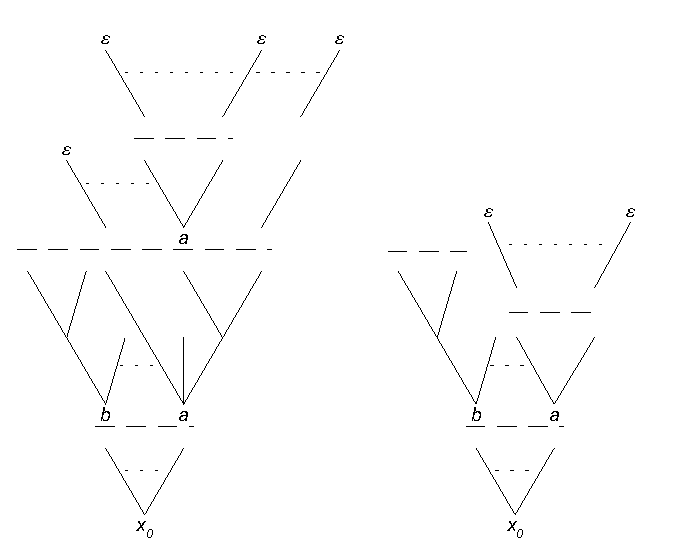
\includegraphics{img/stromy}
    \caption{Vytváranie redukovaného odvodenia} \label{strom}
    \end{figure}

    Označme $m$ dĺžku najdlhšej pravej strany spomedzi všetkých
    pravidiel $G'$ a $n=|V\union\{x_0\}|$. Tvrdíme, že stačí zvoliť:
    \[
    k=3m^n
    \]
    Pre $\forall w\neq\eps,w\in L(G')$ s odvodením $x_0\Ra
    w_0\Ra w_1\Ra\cdots\Ra w_n\equiv w$ bez újmy na všeobecnosti
    predpokladajme, že toto je redukované. Výskyt symbolu $a$ v jednom
    zo slov $w_i$ nazveme neproduktívny $\Longleftrightarrow$ ak tento
    výskyt je návestím koreňa podstromu, ktorého všetky listy majú
    návestie $\eps$. Inak výskyt nazveme produktívny. Pokiaľ
    $w\neq\eps$, tak $w_i$ obsahuje najmenej jeden produktívny
    symbol, navyše počet produktívnych symbolov vo $w_i\leq|w|$. Stačí
    nám ukázať, že $\forall i$, keď $Q$ je podslovo $w_i$ a platí
    $|Q|=3m^n$, potom $Q$ obsahuje najmenej jeden produktívny symbol.
    Pre $i<n$ žiadne podslovo $w_i$ nie je dlhšie ako $3m^n$. Pre
    $i=n+j,j\geq0$ predpokladajme, že $Q$ je podslovo $w_i,|Q|=3m^n$.
    $Q$ môžeme zapísať nasledovne:
    \[
    Q=Q_1Q_2Q_3,|Q_1|=|Q_2|=|Q_3|=m^n
    \]
    Predpokladajme, že $Q$ obsahuje iba neproduktívne symboly.
    Uvažujme nejaký výskyt symbolu $a$ v $Q_2$. Existuje jediný výskyt
    symbolu $b$ vo $w_{i-n}$ taký, že $a$ je návestie v strome $T$,
    ktorého koreň má návestie $b$. Ďalej, voľbou $Q,m,n$ všetky listy
    v $T$ majú návestia $\eps$. To je spor, lebo potom existuje
    v $T$ vetva s dvoma uzlami s rovnakým návestím
\end{dokaz}

\begin{veta}
    (O lineárnom priestore)
    \\ Nech $A$ je Turingov
    stroj\footnote{definície, popis modelu a iné v \cite{Hopc}} (TS)
    taký, že existuje $k$ také, že pre každé slovo $w$ tento TS
    použije pri práci na $w$ najviac $k|w|$ políčok. Potom
    $L(A)\in\mathcal{L}_{ECS}$
\end{veta}

\begin{veta}
    $\mathcal{L}_{OL}\subseteq\mathcal{L}_{ECS}$
\end{veta}

\begin{dokaz}
    Použijeme lemu \ref{linear} a na základe vety o lineárnom
    priestore, ktorá potom pre $OL$-jazyky platí, dostávame
    $L(G)\in\mathcal{L}_{ECS}$
\end{dokaz}

\subsection {Rozšírené $OL$-systémy ($EOL$-systémy)}

Ako sa pri $OL$-systémoch ukázalo, paralelné prepisovanie symbolov
nám istú silu pridalo, no fakt, že do jazyka sme museli zahrnúť
všetko, čo sme vyrobili (každú vetnú formu), nám veľkú časť nášho
optimizmu odobral. $EOL$-systémy nám dovolia opäť (ako pri
gramatikách Chomského hierarchie) filtrovať vetné formy rozdelením
množiny symbolov na terminály a neterminály. Do akej miery sa nám
tým náš model zosilní (malo by byť jasné, že jeho sila bude
minimálne taká, ako sila $OL$-systémov) si ukážeme na príklade
neskôr

\begin{definicia}
    $EOL$-systém je štvorica $G=(N,T,P,w), P\subseteq (N\union
    T)\times(N\union T)^{*}$ a $\forall a\in (N\union T)$ existuje v $P$
    pravidlo
\end{definicia}

\begin{definicia}
    Krok odvodenia je relácia $\Ra$ na $(N\union T)^{*}$ definovaná
    nasledovne: \mbox{$u\Ra v$} práve vtedy, keď $u=a_{1}\dots
    a_{n},\forall i\med a_{i}\in(N\union T),v=b_{1}\dots b_{n},\forall
    i\med b_{i}\in(N\union T)^{*}$ a $\forall i\med a_{i}\ra b_{i}\in P$
\end{definicia}

\begin{definicia}
    Jazyk generovaný $EOL$-systémom $G$ je $L(G)=\{x\in T^{*}\mm
    w\overset{*}\Ra x\}$
\end{definicia}

\begin{priklad}
    $G_{1}=(\{\sigma\},\{a,b\},\{\sigma\ra a,\sigma\ra b,a\ra
    a^{2},b\ra b^{2}\},\sigma)$, potom zjavne jazyk
    $L(G_{1})=\{a^{2^{n}}\mm n\geq0 \}\union\{b^{2^{n}}\mm
    n\geq0\}\not\in\mathcal{L}_{OL}$\\ Tento príklad ukazuje, že
    $EOL$-systémy sú silnejšie ako obyčajné $OL$-systémy a tým sme
    vlastne dali odpoveď na otázku, ktorú sme si položili na začiatku
    kapitoly, v tomto prípade sa sila neterminálu prejavila v tom, že
    nám umožnila spraviť zjednotenie dvoch jazykov
\end{priklad}

\begin{priklad}
    $G_{2}=(\{A\},\{a,b\},\{A\ra A,A\ra a,a\ra a^{2},b\ra b\},AbA)$
    potom jazyk ge\-ne\-ro\-va\-ný $G$ je
    $L(G_{2})=\{a^{2^{n}}ba^{2^{m}}\mm
    m,n\geq0\}\not\in\mathcal{L}_{OL}$
\end{priklad}

\begin{priklad}
    \label{efko}
    $G_{3}=(\{S,A,B,C,\bar{A},\bar{B},\bar{C},F\},\{a,b,c\},P,S)$
    \begin{tabbing}
    \= xxx \= $P=\{\med$ \= xxxxxxxxxx \= xxxxxxxxxx \= xxxxxxxxxx
    \= xxxxxxxxxx
    \kill
    \> \> $P=\{\med$ \> $S\ra ABC$ \> $a\ra F$ \> $b\ra F$ \> $c\ra
    F$\\
    \> \> \> $A\ra A\bar{A}$ \> $A\ra a$ \> $\bar{A}\ra\bar{A}$ \> $\bar{A}\ra
    a$\\
    \> \> \> $B\ra B\bar{B}$ \> $B\ra b$ \> $\bar{B}\ra\bar{B}$ \> $\bar{B}\ra
    b$\\
    \> \> \> $C\ra C\bar{C}$ \> $C\ra c$ \> $\bar{C}\ra\bar{C}$ \> $\bar{C}\ra
    c$\\
    \> \> \> $F\ra F\med\}$
    \end{tabbing}
    Možno niekoho prekvapí fakt, že $L(G_{3})=\{a^{n}b^{n}c^{n}\mm
    n\geq1\}$, no ak sa nad systémom $G_{3}$ trošku zamyslíme, tak sa
    nám táto skutočnosť ihneď vyjasní. Ide tu totiž o rafinované
    využitie neterminálu $F$ na to, aby terminálne slová vznikali
    naraz (teda slová z jazyka $L(G_{3})$ vznikajú v jednom kroku
    odvodenia prepísaním všetkých neterminálov na terminálne symboly).
    Ako si v nasledovnej vete ukážeme, tento jav nie je ani zďaleka
    taký zriedkavý, ako by sa mohlo zdať
\end{priklad}

\begin{veta}(Synchronizovaný tvar $EOL$-systému)
    \\ Nech $G=(N,T,P,w)$ je $EOL$-systém pre jazyk $L$. Potom existuje
    taký $EOL$-systém $G'$, $L(G')=L(G)$, že všetky jeho terminálne
    slová vznikajú z neterminálnych vetných foriem v jednom kroku
    odvodenia\footnote{teda keď sa vo vetnej forme objaví prvý
    terminál, tak nutnou podmienkou, aby sme niekedy vygenerovali
    terminálne slovo je, aby v kroku odvodenia, kedy sa do vetnej
    formy dostal, ``zterminálnela'' vetná forma celá}
\end{veta}

\begin{dokaz}
    Ukážeme konštrukciu synchronizovaného $EOL$-systému $G'$. Najskôr
    si vytvoríme nové neterminály, ktoré budeme potrebovať:
    \begin{itemize}
    \item $\forall a\in T$ vytvoríme $\xi_a$ (ak $a,b\in T$, tak
    $\xi_a\neq\xi_b$)
    \item $F,\sigma'$, budú predstavovať FALSE, resp. nový počiatočný
    symbol
    \end{itemize}
    Označme $N'=\{\xi_a\mm a\in T\}$. Pre jednoduchosť zaveďme
    niekoľko pojmov, ktoré neskôr využijeme:
    \begin{enumerate}
    \item Nech $S$ je ľubovoľná množina reťazcov z $(N\union T)^*$, pre
    ňu definujeme množinu $A(S)$ nasledovne:
    \begin{enumerate}
    \item reťazec $b_{1}\dots b_{n}\in A(S)\overset{def}
    \Longleftrightarrow$ ak existuje reťazec $a_{1}\dots a_{n}\in S$
    taký, že buď $b_i=a_i$ alebo $a_i\in T$ a $b_i=\xi_i$ (teda
    $b_i\in N'$), potom $A(S)\subset(N\union N'\union T)^*$
    \item ak $S\neq\emptyset$, potom $A(S)\neq\emptyset$, lebo
    $S\subseteq A(S)$
    \end{enumerate}
    \item $\delta_P(a)$ nazveme množinu všetkých pravých strán
    pravidiel pre symbol $a$ z $P$
    \end{enumerate}
    Definujme synchronizovaný $EOL$-systém $G'$ nasledovne: $G'=(N\union
    N'\union\{F,\sigma'\},T,P',\sigma')$, pričom
    \begin{tabbing}
    \= xxx \= $P'\med$: \= xxxxxxxxxxxxxxxx \= xxxxxxxxxxx \kill \>\>
    $P':$ \> $\delta_{P'}(\sigma')=A(\{w\})$\\ \>\>\> $\forall
    a\in(T\union \{F\})$ \> $(a\ra F)\in P'$\\ \>\>\> $\forall a\in N$
    \> $\delta_{P'}(a)=A(\delta_P(a))$\\ \>\>\> $\forall\xi_a\in N'$
    \> $\delta_{P'}(\xi_a)=A(\delta_P(a))$
    \end{tabbing}
    Malo by byť zrejmé, že teminálne slová musia v $G'$ vznikať naraz,
    pretože ak sa náhodou nejaký terminál do venej formy dostane skôr
    ako ostatné, tak sa v ďaľšom kroku prepíše nutne na $F$ a z $F$ sa
    už nikdy terminál nestane. Rovnako zrejmé by malo byť
    $L(G')=L(G)$, pretože nové neterminály $\xi_i$ vo vetnej forme
    akoby nahrádzali terminálne symboly, a tak simulovali odvodenie v
    pôvodnom systéme $G$
\end{dokaz}

\begin{veta}
    Každý konečný jazyk je v $\mathcal{L}_{EOL}$
\end{veta}

\begin{dokaz}
    Nech $L$ je konečný, potom existuje regulárna gramatika $G$ taká,
    že $L=L(G)$. Táto regulárna gramatika je ale zároveň (po doplnení
    pravidiel $a\ra a\med\forall a\in(N\union T)$) aj hľa\-da\-ným
    $EOL$-systémom
\end{dokaz}

\begin{lema}
    \label{norm_tvarEOL} Nech $G$ je $EOL$-systém, potom existuje
    $EOL$-systém $G'$, ktorého všetky pravidlá obsahujúce $a\in T$ na
    ľavej strane sú tvaru $a\ra a$
\end{lema}

\begin{dokaz}
    Zkonštruujeme $EOL$-systém $G'$ nasledovne: pre každé $a\in T$
    zavedieme nový neterminál $\xi_{a}$ a upravíme pravidlá:
    \begin{enumerate}
    \item tie pravidlá, kde sa vyskytujú terminály, nahradíme novými tak,
    že všetky terminály (na ľavej i pravej strane) zmeníme na
    príslušné nové neterminály ($a\in T$ nahradíme $\xi_{a}\in N$)
    \item pre každé $a\in T$ pridáme pravidlo $a\ra a$
    \item pre každé nové $\xi_{a}\in N$ pridáme pravidlo $\xi_{a}\ra a$
    \end{enumerate}
\end{dokaz}

\begin{veta}
    Trieda $\mathcal{L}_{EOL}$ je uzavretá na
    $\union,\cdot,+,\intersect\mathcal{R},h_{\eps}$ a nie je uzavretá
    na $h^{-1}$
\end{veta}

\begin{dokaz}
    Dokážeme iba dve vlastnosti, väčšina ostatných dôkazov sa až na
    malé technické detaily veľmi nelíši od známych konštrukcií pre
    bezkontextové gramatiky:
    \begin{itemize}
    \item $\union :$ Máme $EOL$-systémy $G_{1}$ pre $L_{1}$ a $G_{2}$
    pre $L_{2}$. Ku $G_{1},G_{2}$ spravíme normálne tvary
    $G'_{1},G'_{2}$ podľa konštrukcie z lemy \ref{norm_tvarEOL}. Bez
    ujmy na všeobecnosti môžeme predpokladať, že $N'_{1}\intersect
    N'_{2}=\emptyset$. Vytvoríme $G_{3}$ pre $L_{1}\union L_{2}$
    nasledovne: zavedieme nový neterminál $\sigma_{3}$ tak, že
    $\sigma_{3}\not\in N'_{1}$ \mbox{a $\sigma_{3}\not\in N'_{2}$}.
    Ďalej $N_{3}=N'_{1}\union N'_{2}\union\{\sigma_{3}\}$,
    $T_{3}=T'_{1}\union T'_{2}$, $P_{3}=P'_{1}\union
    P'_{2}\union\{\sigma_{3}\ra\sigma'_{1}|\sigma'_{2}\}$ \mbox{a
    nakoniec} $G_{3}=(N_{3},T_{3},P_{3},\sigma_{3})$
    \item $h^{-1} :$ Zoberme jazyk $L\in\mathcal{L}_{EOL},
    L=\{a^{2^n}\mm n\geq0\}$ a definujme homomorfizmus $h$ nasledovne:
    $h(a)=a, h(b)=\eps$. Potom $h^{-1}(L)=\{w\in\{a,b\}^*\mm
    \#_a w=2^n,n\geq0\}$. Ukážeme, že
    $h^{-1}(L)\not\in\mathcal{L}_{EOL}$. Nech $G$ je $EOL$-systém pre
    $h^{-1}(L)$. Zoberme $w_0\in h^{-1}(L)$, nech $\#_a w_0=n$.
    Zoberme ľubovoľné dve $a$, medzi ktorými sú iba $b$. Ak je medzi
    týmito dvoma $a$ ``príliš veľa''\footnote{tento počet vieme určiť,
    závisí napr. od dĺžky najdlhšej pravej strany pravidla v $G$,
    bližšie v \cite{clos}} $b$, tak takéto slovo nedokážeme vyrobiť
    (nemáme na to dostatok času), čo je spor s tým, že $G$ je
    $EOL$-systém pre $h^{-1}(L)$
    \end{itemize}
\end{dokaz}

\begin{veta}
    $\mathcal{L}_{CF}\subsetneq\mathcal{L}_{EOL}$
\end{veta}

\begin{dokaz}
    Každá bezkontextová gramatika vyhovuje definícii $EOL$-systému (po
    doplnení pravidiel $a\ra a\med\forall a\in(N\union T)$), teda platí
    nevlastná inklúzia $\mathcal{L}_{CF}\subseteq\mathcal{L}_{EOL}$.
    Že platí aj vlastná inklúzia, sme ukázali v príklade \ref{efko},
    kde sme našli $EOL$-systém pre jazyk $L=\{a^{n}b^{n}c^{n}\mm
    n\geq1\}\in\mathcal{L}_{CS} - \mathcal{L}_{CF}$
\end{dokaz}

\begin{poznamka}
    $1L$ a $2L$-systémy sú nejakou analógiou kontextových gramatík, i
    keď o ich sile by sa dali viesť podobné diskusie ako pri
    $OL$-systémoch. Snáď len toľko, že obojstranný kontext je silnejší
    ako jednostranný a oba systémy sú silnejšie ako $OL$-systémy
\end{poznamka}

\subsection{$TOL$-systémy (table)}

Tieto systémy nebudeme striktne definovať, povieme si len základné
veci, ktorými sa od kla\-sic\-kých $OL$-systémov odlišujú.
$TOL$-systém $G=(V,P_{1},\dots,P_{k},w_{0})$ má niekoľko
(konkrétne $k$) sád pravidiel, v danom kroku odvodenia použijeme
na vetnú formu iba jednu sadu pravidiel

\begin{priklad}
    $G=(\{a\},\{a\ra a^{2}\},\{a\ra a^{3}\},a)$, potom
    $L(G)=\{a^{2^{n}}a^{3^{m}}\mm n,m\geq0\}\not\in\mathcal{L}_{OL}$
\end{priklad}

\begin{poznamka}
    Trieda $\mathcal{L}_{TOL}$ zdieľa ``zlé'' uzáverové vlastnosti
    triedy $\mathcal{L}_{OL}$. Podobne ako pre $\mathcal{L}_{OL}$
    platí aj pre $\mathcal{L}_{TOL}$ vzťah
    $\mathcal{L}_{TOL}\subseteq\mathcal{L}_{ECS}$
\end{poznamka}

\section{Ďaľšie paralelné gramatiky}

\subsection{Indické paralelné gramatiky}

\begin{definicia}
    Indická paralelná gramatika (IP) je štvorica $G=(N,T,P,\sigma)$,
    pričom \mbox{$\sigma\in N$} $N\intersect T=\emptyset, P\subseteq
    N\times(N\union T)^{*}$
\end{definicia}

\begin{definicia}
    Krok odvodenia IP $G$ je relácia $\Ra$ keď sa všetky výskyty
    zvoleného neterminálu prepíšu naraz tým istým pravidlom
\end{definicia}

\begin{priklad}
    $G_{1}=(\{\sigma\},\{a\},\{\sigma\ra\sigma\sigma,\sigma\ra
    a\},\sigma)$ potom $L(G_{1})=\{a^{2^{n}}\mm n\geq0\}$
\end{priklad}

\begin{priklad}
    Dyckov jazyk nad dvoma písmenkami $D_{1}$ (jazyk správne
    uzátvorkovaných výrazov) nie je $\mathcal{L}_{IP}$
\end{priklad}

\begin{dokaz}
    Sporom predpokladajme, že $D_{1}\in\mathcal{L}_{IP}$, potom
    existuje IP gramatika $G$ taká, že \mbox{$L(G)=D_{1}$}. Ukážeme,
    že by musela mať nekonečne veľa neterminálov, čo nie je možné. Pre
    jednoduchosť označme $L=D_{1}$. Vytvoríme v $L$ hierarchiu tvarov
    slov nasledovne: definujme rekurentne podmnožiny $L$ a uvedomme
    si, koľko najmenej neterminálov treba na generovanie slov z každej
    z nich:
    \begin{description}
    \item{$\med$} $L_{1}=\{\med a^{n}b^{n}\mm n\geq1\med\}^{+}$ treba aspoň 2
    neterminály
    \item{$\med$} $L_{i+1}=\{\med a^{n}wb^{n}\mm w\in L_{i},n\geq1\med\}^{+}$
    treba aspoň $i+2$ neterminálov
    \end{description}
    Ako vidno, táto hierarchia je nekonečná, teda na generovanie
    $(\bigcup_{i=1}^{\infty}L_{i})\subseteq L$ je treba nekonečne veľa
    neterminálov
\end{dokaz}

\begin{veta}
    $\mathcal{L}_{IP}\intersect\mathcal{L}_{CF}=\mathcal{L}_{DBL}$
\end{veta}

\begin{poznamka}
    $\mathcal{L}_{DBL}$ je trieda {\it Derivation Bounded Languages},
    ku každému jazyku z tejto triedy existuje $k$ také, že počet
    neterminálov v každej vetnej forme je menší ako $k$
\end{poznamka}

\begin{veta}
    $\mathcal{L}_{IP}\subseteq\mathcal{L}_{ECS}$
\end{veta}

\begin{veta}
    $\mathcal{L}_{IP}$ je uzavretá na $\union,\cdot,*,h$
\end{veta}

\begin{veta}
    $\mathcal{L}_{IP}$ je neporovnateľná s $\mathcal{L}_{EOL}$
\end{veta}

\begin{veta}
    $\mathcal{L}_{IP}\subseteq\mathcal{L}_{ETOL}$ (extended $TOL$)
\end{veta}

\subsection{Ruské paralelné gramatiky}

\begin{definicia}
    Ruská paralelná gramatika je pätica $G=(N,T,P_{1},P_{2},\sigma)$,
    pričom $\sigma\in N$, \mbox{$N\intersect T=\emptyset$}, $P_{1}, P_{2}$
    sú konečné množiny pravidiel, $P_{1},P_{2}\subseteq N\times(N\union
    T)^{*}$
\end{definicia}

\begin{definicia}
    Krok odvodenia: všetky výskyty zvoleného neterminálu sa prepíšu
    naraz istým pravidlom z $P_{1}$, alebo sa prepíše práve jeden
    neterminál pravidlom z množiny $P_{2}$
\end{definicia}

\subsection{Absolútne paralelné gramatiky}

\begin{definicia}
    Absolútne paralelná gramatika (AP) je štvorica $G=(N,T,P,\sigma)$,
    kde \mbox{$\sigma\in N$}, $N\intersect T=\emptyset$, $P$ je konečná
    množina pravidiel tvaru
    $(A_{1},\dots,A_{n})\ra(w_{1},\dots,w_{n})$, kde \mbox{$\forall
    A_{i}\in N$}, $w_{i}\in(N\union T)^{*}$
\end{definicia}

\begin{definicia}
    Krok odvodenia je relácia $w\Ra v$ práve vtedy, keď
    $w=u_{1}A_{1}u_{2}A_{2}\dots u_{n}A_{n}u_{n+1}$ \mbox{a
    $v=u_{1}w_{1}u_{2}w_{2}\dots u_{n}w_{n}u_{n+1}$}, pričom
    $u_{1},\dots u_{n+1}\in T^{*}$ (t.j. naraz prepisujeme všetky
    neterminály vo vetnej forme, na každú možnosť výskytu neterminálov
    musíme mať pravidlo)
\end{definicia}

\begin{priklad}
    Pozrime sa na AP gramatiku:\\
    $G=(\{S\},\{a,b,c\},\{(S)\ra(SSS),(S,S,S)\ra (aS,bS,cS),(S,S,S)\ra
    (a,b,c)\},S)$ potom $L(G)=\{a^{n}b^{n}c^{n}\mm n\geq1\}$
\end{priklad}

\begin{veta}
    $\mathcal{L}_{AP}$ je $\mathcal{AFL}$
\end{veta}

\begin{veta}
    $\mathcal{L}_{AP}\intersect 2^{a^{*}}\subseteq\mathcal{R}$ (t.j.
    jednopísmenkové $AP$ jazyky sú regulárne)
\end{veta}

\begin{dokaz}
    Nech $L\in\mathcal{L}_{AP}$ a $G=(N,T,P,A_p)$ je $AP$ gramatika
    taká, že $L(G)=L$. Bez újmy na všeobecnosti môžeme predpokladať,
    že $T=\{a\}$. Nech \mbox{$N=\{A_1,\dots,A_n\}$}. Definujme $N'$
    nasledovne: $N'=\{A_p\}\union\{A_{i_1,\dots,i_k}\mm\forall j\med
    A_{i_j}\in N,\med A_{i_1},\dots,A_{i_k}$ sa nachádzajú na pravej
    strane niektorého (rovnakého) z pravidiel $P$ v tomto poradí$\}$.
    Bez újmy na všeobecnosti môžeme pred\-pokla\-dať, že všetky
    pravidlá z $P$ sú tvaru
    $(A_{i_1},\dots,A_{i_m})\ra(a^{k_1}\pi_1,\dots,a^{k_m}\pi_m)$, kde
    $\forall i\med \pi_i\in N^*$. Definujme
    $\varphi_i=i_1,\dots,i_l\Longleftrightarrow\pi_i=A_{i_1}\dots
    A_{i_l}$ Vytvoríme množinu pravidiel $P'$ nasledovne:
    \[
    A_{i_1,\dots,i_k}\ra
    a^{w_1+\cdots+w_k}A_{\varphi_{i_1},\dots,\varphi_{i_k}}\in
    P'\Longleftrightarrow
    (A_{i_1},\dots,A_{i_k})\ra(a^{w_1}\pi_1,\dots,a^{w_k}\pi_k)\in P
    \]
    Teraz definujme $G'=(N',\{a\},P',A_p)$. $G'$ je zrejme regulárna
    gramatika a z konštrukcie vyplýva, že $L(G')=L(G)$
\end{dokaz}

\begin{veta}
    $\mathcal{L}_{AP}=\mathcal{L}_{2DAP}$
\end{veta}

\begin{poznamka}
    $\mathcal{L}_{2DAP}$ je trieda jazykov, ktoré sú generované
    dvojsmernými determi\-nis\-tic\-ký\-mi $a$-prek\-la\-dač\-mi
\end{poznamka}
